\documentclass[11pt]{article}
\usepackage{fontspec}
\IfFontExistsTF{TeX Gyre Termes}{\setmainfont{TeX Gyre Termes}}{\IfFontExistsTF{Times New Roman}{\setmainfont{Times New Roman}}{\setmainfont{lmroman10}[Extension=.otf,UprightFont=*-regular,BoldFont=*-bold,ItalicFont=*-italic,BoldItalicFont=*-bolditalic]}}
\IfFontExistsTF{TeX Gyre Heros}{\setsansfont{TeX Gyre Heros}}{\setsansfont{lmsans10}[Extension=.otf,UprightFont=*-regular,BoldFont=*-bold,ItalicFont=*-oblique,BoldItalicFont=*-boldoblique]}
\usepackage[numbers,sort&compress]{natbib}
\usepackage{microtype}
\usepackage{booktabs}
\usepackage{graphicx}
\usepackage{tabularx}
\usepackage{float}
\usepackage{hyperref}
\usepackage{memmy-review}
\hypersetup{colorlinks=true,linkcolor=MemmyAccent,citecolor=MemmyAccent,urlcolor=MemmyAccent}
\renewcommand{\memmyreviewlabel}{LITERATURE REVIEW}
\renewcommand{\memmyabstractlabel}{Abstract}
\renewcommand{\memmygeneratedby}{Generated with the Memmy Literature Review Plugin}
\renewcommand{\memmydisclaimer}{AI-generated; reference only; formal submission unsupported.}
\renewcommand{\memmyfullnotice}{This AI-generated literature review is for reference only and is not intended or supported for formal academic submission. The user must independently verify all facts, citations, and references.}
\title{Long-Term Agent Memory: From Evidence to Evolving Knowledge}
\begin{document}
\maketitle

\begin{abstract}
This sample demonstrates the Memmy literature review layout through the topic of long-term agent memory. It presents source management, evidence organization, retrieval, and revision using hierarchical headings, prose, a workflow diagram, a comparison table, and citations. The content and reference entry are illustrative and do not constitute research evidence.
\end{abstract}

\section{From information to traceable memory}

Long-term memory organizes scattered interactions and research materials into knowledge that can be retrieved, checked, and revised. For a literature review, a fluent summary is only a starting point. Readers also need to know where a claim comes from, the conditions under which it applies, and how it should change when new evidence appears.

A clear workflow connects source ingestion, evidence indexing, retrieval and synthesis, and revision. Linked records allow readers to trace a statement back to its source. The diagram on this page illustrates the layout; it does not report experimental results.

\begin{figure}[H]
\centering
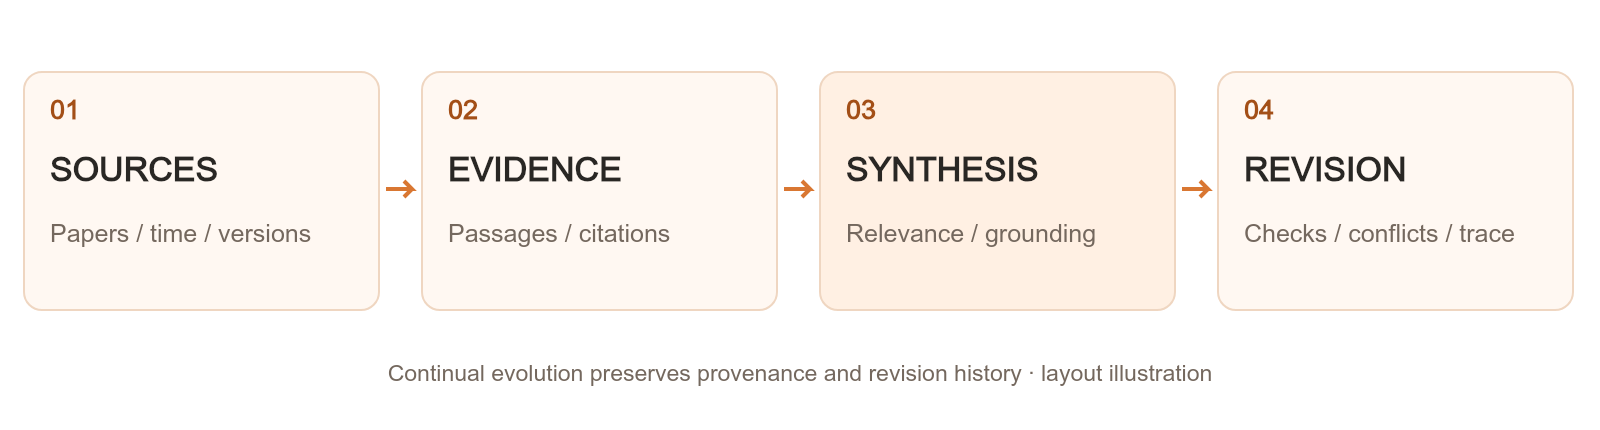
\includegraphics[width=0.92\linewidth,height=0.45\textheight,keepaspectratio]{assets/figures/lifecycle-source.png}
\caption{A memory workflow from sources to revision. This is a layout illustration, not an experimental result.}
\label{fig:lifecycle-block}
\end{figure}

\section{Design choices for memory systems}

Memory design balances retrieval quality, update cost, and interpretability. Original passages support verification, structured relations organize connections across papers, and condensed summaries support browsing. These representations can be combined according to the task and available evidence.

\subsection{Retrieval and evidence grounding}

Retrieval should preserve both content and provenance while passing explicit evidence boundaries to writing. Synthesis should distinguish direct observations, comparisons across papers, and judgments that still require verification. Agreement between sources must be interpreted in light of time, scope, and experimental conditions.

\subsection{Conflict resolution and versioning}

When sources differ, preserving revision relationships is more informative than silently replacing an earlier conclusion. Version records should identify the new evidence, affected claims, and reason for change. This supports historical recovery and makes later audits easier to interpret.

\section{Evaluation and open questions}

Evaluation should examine source completeness, verifiable claims, preserved revision history, and consistency between citations and prose. The illustrative table compares three common organizational approaches. Its entries are provided for layout demonstration only.

Open questions concern long-term maintenance and reuse across tasks: detecting stale information, preserving evidence diversity within a reasonable cost, and communicating the scope of conclusions. An actual review should replace these demonstration paragraphs with independently verified evidence \cite{LayoutDemo2026}.

\begin{table}[H]
\centering
\small
\caption{Illustrative comparison of memory representations (layout demonstration).}
\label{tab:comparison-block}
\begin{tabularx}{\linewidth}{>{\hsize=0.633\hsize\linewidth=\hsize\raggedright\arraybackslash}X >{\hsize=1.267\hsize\linewidth=\hsize\raggedright\arraybackslash}X >{\hsize=1.100\hsize\linewidth=\hsize\raggedright\arraybackslash}X}
\toprule
\rowcolor{MemmyTint} \textbf{Representation} & \textbf{Primary use} & \textbf{Maintenance focus} \\
\midrule
Original passages & Preserve context for verification & Source and version identifiers \\
Structured relations & Connect entities and findings & Relation updates and conflicts \\
Summaries and indexes & Browse topics and locate evidence & Freshness and evidence grounding \\
\bottomrule
\end{tabularx}
\end{table}

\begin{thebibliography}{99}
\small
\raggedright
\setlength{\itemsep}{0.18em}
\setlength{\parsep}{0pt}
\bibitem{LayoutDemo2026} Memmy. (2026). Layout demonstration entry (not a real publication)
\end{thebibliography}
\end{document}
